%------------------------------------------------------------------------------
\chapter{Research Paper: Measuring the quality of relational to RDF mappings}
\label{sec:app_rdb2rdf}
%------------------------------------------------------------------------------

\section{Abstract}
Mapping between relational data and linked data (RDB2RDF) is an essential prerequisite for evolving the World Wide Web into the Web of Data.
We propose a methodology to evaluate the quality of such mappings against a set of objective metrics.
Our methodology, whose key principles have been approved by a survey among RDB2RDF experts, can be applied to evaluate both automatically and manually performed mappings regardless of their representation.
The main contributions of the paper are: (1) assessing the quality requirements for mappings between relational databases and RDF, and (2) proposing methods for measuring how well a given mapping meets the requirements.
We showcase the usage of the individual metrics with illustrative examples from a real-life application.
Additionally, we provide guidelines to improve a given mapping with regard to the specific metrics. 

\section{Introduction}

Translating the data stored in relational databases (RDB) to the linked data format is an essential prerequisite for evolving the current Web of documents into a Web of Data.
In order to be effectively and efficiently reusable, linked data should meet certain data quality requirements~\cite{Zaveri}.
Assessing the quality of a linked dataset created from RDB may be a laborious, repetitive task if the dataset is frequently recreated from its RDB source, e.g.\ after any update to the RDB.
We therefore claim that it is possible to positively influence the quality of a linked dataset created from RDB by improving the quality of the RDB2RDF \emph{mapping} that produces the linked data\footnote{Here, we use the term ``mapping'' to refer to the function that maps relational database columns to RDF properties, but not to materialisations of such mappings in concrete languages or representations, nor to tools that would execute such a function.}.
To the best of our knowledge there has not been prior research towards collecting and describing quality requirements for RDB2RDF mappings.
Thus, this paper aims to fill the gap by providing a system of metrics to measure the quality of RDB2RDF mappings.

A large number of tools for mapping relational data to RDF exist already\footnote{One of the listings is available at \url{https://github.com/timrdf/csv2rdf4lod-automation/wiki/Alternative-Tabular-to-RDF-converters}.}; they implement different mapping approaches, often allowing to customize the mapping.
To standardize the description of mappings, the W3C RDB2RDF Working Group has released two recommendations in 2012 (more details in~ Section\ref{sec:mapping-quality}): Direct Mapping~\cite{direct_mapping}, which produces RDF graph representations directly from a relational database (data and schema) and the Relational Database to RDF Mapping Language (R2RML)~\cite{r2rml} for expressing customized mappings.
 
In this paper, we aim at developing a system of quality metrics that can be applied both to direct and customized mappings that works with different representations of mappings (R2RML or proprietary formats, visual diagrams, tables, etc.).
Any of these representations are suitable for being evaluated with the proposed system as long as one can derive a list of database columns (including unmapped ones) and their corresponding RDF properties (for mapped ones).

To determine the scope of requirements that can be posed to RDB2RDF mappings, we studied the state of the art in related research fields such as ontology matching, linked data quality assessment and RDB2XML mappings. 
However, as Section~\ref{related_work} shows, these metrics collected from the scientific community do not solve the given problem entirely.
In order to fulfil the list, we followed the Direct and R2RML Mapping recommendations.
Some of the RDB2RDF features standardized in the documents are connected with the output data quality dimension, while others influence the quality of the mapping itself. 
For example, the ability to define R2RML views allows to incorporate domain semantics into the mapping – an opportunity that we consider to increase the quality of mapping.
We propose not only a system of metrics but also define means of measuring them, along with guidelines to improve the rating of a dataset w.r.t.\ each metric.

The paper is structured as follows: in Section~\ref{related_work} we discuss the existing approaches, in Section~\ref{requirements} we summarize the quality requirements for mappings and the metrics for measuring the quality.
\hyperref[evaluation]{Section~\ref*{evaluation}} presents the results of the survey conducted in order to collect the community feedback.
In Section~\ref{conclusions}, we conclude and propose future research directions.

\section{Related work}
\label{related_work}

\paragraph{RDB2RDF mapping approaches.}
Although previous research has not explicitly focused on collecting requirements for RDB2RDF mappings, many such requirements can be found in best practice and mapping approach descriptions.
For instance, in \cite{hillairet2008mde}, the importance of reusing existing vocabularies to enhance the interoperability of the output dataset is explained.
We extend this statement to a set of requirements combined in the \emph{interoperability} dimension, taking into account not only quantitative, but also qualitative metrics.

We notice that existing literature on the topic uses incoherent terminology.
Often, the term \emph{mapping} is used instead of mapping \emph{language}, e.g.\ in~\cite{Auer2010,Erling2008}. 
Discussing the requirements for mapping \emph{language}, both articles mention the following requirements for RDB2RDF \emph{mapping} as well:

\begin{itemize}
\item presence of both ETL and on-demand implementation
\item incorporating domain semantics that is often implicit or not captured at all in the RDB schema
\item indication of time metadata about the dataset during the mapping creation process to control the dataset currency (we subsume this metric under “data quality”)
\item intensive reuse of the existing ontologies
\end{itemize}    

\paragraph{Requirements for mappings between relational data and XML.}
The topic of mapping relational data to \emph{XML} is related to RDB2RDF mapping due to the similarity between the XML and RDF data models.
The earliest articles on the quality of RDB2XML mappings (e.g.~\cite{Schmidt, Shanmugasundaram}) only take into account the performance of the mapping algorithms.
This is because RDB2XML mappings are mostly produced automatically and do not allow customization.
Only few authors (e.g.~\cite{sahuguet2001everything}) propose metrics for evaluating the quality of the output data.
However, the proposed metrics evaluate only the syntactic correctness of the output XML and therefore cannot be applied to documents in RDF (except for \emph{presence of syntax errors}).

Other approaches (e.g.\ \cite{he1999relational}) prove the need for customizable techniques of mapping due to the wide gap between these two formats.
As their major evaluation criterion, they use the \textit{efficiency of query processing}.
We adopt this approach and base our \textit{simplicity} metric on it.
Liu et al.~\cite{liu2006designing} describe an approach to design a high-quality XML Schema from ER diagrams.
The authors define a list of requirements for the design; the most relevant one for our purposes is \emph{information preservation}.
However, the metrics for \emph{measuring} such requirements are not discussed.
We study the information preservation requirement in detail and provide objective metrics in the \emph{Faithfulness of Output} dimension.

\paragraph{Requirements for ontology matching.}
Mapping between a database schema and an RDF vocabulary can also be viewed as a special case of ontology matching.
Several studies propose requirements for measuring the quality of an ontology matching.
According to~\cite{euzenat2007ontology}, all proposed measures can be distinguished between compliance measures, measures concerned with system usability and performance measures focusing on runtime or memory usage.
As our study focuses on evaluating the quality of mapping itself, we do not take the system usability or performance dimensions into account.

In the evaluation of ontology matching, compliance measures are based on the two classical information retrieval measures of \emph{precision} and \emph{recall}~\cite{vanRijsbergen}.
We adapt these metrics to the evaluation of RDB2RDF mappings and include them in the \emph{faithfulness of output} dimension as \emph{coverage} and \emph{accuracy of data presentation} metrics. 

\paragraph{Measuring linked data quality.}
The quality of mapping correlates with the quality of output linked data produced by the mapping.
Poor design decisions made at the stage of defining a mapping, such as using deprecated classes, redundant attributes or badly formed URIs, decreases the quality of the output data.
Therefore, metrics for the quality of the output data can be viewed as metrics for quality of the mapping.

The field of assessing the quality of linked data is still in its infancy, but several articles have addressed it already. 
Our recent survey~\cite{Zaveri} collects and compares the existing papers, 
the most complete and detailed ones being Bizer's PhD thesis~\cite{bizer2007quality}, Flemming's master's thesis~\cite{flemming} and empirical evaluations by Hogan et al.\ \cite{hogan2010weaving, hogan2012empirical}. 
The survey provides formal definitions of data quality dimensions and metrics as well as evaluates existing tools for (semi-)automatic measurement of linked data quality.

The current paper assumes that the quality of a linked dataset is influenced by the mapping that produces it and thus categorizes the metrics from the survey from the perspective of the RDB2RDF mapping.
We select those metrics that are related to the mapping process and adapt them to the RDB2RDF domain.


\section{Quality Requirements}
\label{requirements}

This section gives a detailed overview of the proposed quality requirements for RDB2RDF mappings, ways of measuring them (metrics) and guidelines for improving mappings w.r.t.\ these metrics.
Our proposed system incorporates four quality dimensions with 14 objective metrics overall.
For assessing the overall quality of a mapping, one would, in practice, assign \emph{weights} to the metrics.
Their choice depends on the goal of the mapping process.
For example, when the goal of the mapping is to accurately represent the relational data,
the metrics in the “faithfulness of the output” dimension should be assigned the highest weight.

\begin{table*}[!ht]

	\centering		
	\begin{tabulary}{\textwidth}{LLL}
	\toprule
		\textbf{{Requirement}} & \textbf{{Description}} & \textbf{{Measure}} \\
		\midrule
		
		\multicolumn{3}{c}{\textbf{Quality of the mapping implementation and representation}} \\
\hline
		\textbf{Data accessibility} &
Describes how the mapping result can be accessed. 
		 & ETL/on-demand/both\\
\hline
		\textbf{Standard compliance} &
Characterizes if the mapping representation is standard compliant.
		 & boolean \\
\hline
		 
		\multicolumn{3}{c}{\textbf{Faithfulness of the output}} \\		
\hline
		\textbf{Coverage} & Characterizes the mapping completeness  & percentage of DB columns mapped  \\
\hline
		\textbf{Accuracy of data representation} & Characterizes the mapping correctness & percentage of correctly mapped DB columns \\
\hline
		\textbf{Incorporation of domain semantics} & Shows level of domain semantics incorporation & percentage of properties that link to the results of SQL queries \\
\hline
		
		\multicolumn{3}{c}{\textbf{Quality of the output}} \\		
\hline
		\textbf{Simplicity} & Shows the simplicity of SPARQL queries returning the frequently demanded values & percentage of complex SQL queries results integrated into the mapping \\
\hline
		\textbf{Data quality} & Characterizes the quality of output data & aggregation of linked data quality metrics ($\to$ \autoref{tab:data_quality_groups})\\
\hline
		\textbf{Data integration} & Characterizes the interlinking degree of the output data & percentage of external instances integrated into the resultant dataset\\	
\hline
		
		\multicolumn{3}{c}{\textbf{Interoperability}} \\		
\hline
		\textbf{Reuse of existing ontologies} & Shows the amount of reused vocabulary elements & percentage of reused properties and classes\\
\hline
		\textbf{Quality of reused vocabulary elements} & Characterizes the quality of chosen for reuse properties and classes & accumulated quality and popularity of reused vocabulary elements \\
\hline
		\textbf{Accuracy of reused properties} & Characterizes the accuracy of properties reuse & percentage of accurately reused properties \\
\hline
		\textbf{Accuracy of reused classes} & Characterizes the accuracy of classes reuse & percentage of accurately reused classes  \\
\hline
		\textbf{Quality of declared classes/properties} & Shows the quality of ontology documentation & accumulated quality of declared classes/properties\\
\hline
	
	\end{tabulary}
		
	\caption{Summary table of proposed metrics system}
	\label{tab:summarytable}
\end{table*}

\subsection{Quality of the mapping implementation and representation}
\label{sec:mapping-quality}
The requirement of mapping quality implementation and representation combines the requirements for resultant data accessibility and standard compliance of the mapping representation.

\paragraph{Data accessibility.}
Data accessibility describes how the result of the mapping is accessed. 
This metric is also known in the literature as “access paradigm”, “mapping implementation” or “data exposition”~\cite{spanos2012bringing}.
There are two possibilities: (i) Extract Transform Load (ETL) and (ii) on-demand mapping.
According to~\cite{Erling2008}, ETL means physically storing triples produced from relational data in an RDF store.
The disadvantage of ETL is that that, whenever the RDB is updated, you have to re-run the entire ETL process, even if just one RDB record has changed, carrying out an often redundant synchronization process.
However, in the ETL case nothing more than the RDF store is needed to answer a query.

On-demand mapping is realized by translating a SPARQL query into one or more SQL queries at query-time, evaluating these against (a set of) unmodified relational database(s) and constructing a SPARQL result set from the result sets of such SQL queries.
In contrast to the ETL implementation, on-demand mapping requires more resources for processing each query.
However, the on-demand implementation does not face the synchronization issue and does not replicate the data.  
In the light of these advantages and disadvantages, we claim that the best solution is to implement a mapping with both data access approaches.
Thus, the index of implementation takes a value equal to 1, if both implementations are present and 0.5 otherwise.


\paragraph{Standard compliance.}

An RDB2RDF mapping can either be represented as a set of customized rules or through a generic set of rules (as defined by the W3C Direct Mapping standard~\cite{direct_mapping, Bertails_2011}).
Often, the output of a Direct Mapping may not be useful, that is, it may not adequately take the structural/semantic complexity of the database schema into account.
Thus, while the applicability of a Direct Mapping satisfies the requirements for the “standard representation” metric, not using the customized rules will lead to a loss of points w.r.t.\ other metrics.

Languages for representing customized mappings have been surveyed in~\cite{spanos2012bringing}.
Until recently, no standard representation language for RDB2RDF mappings existed, however, as of 2012, R2RML~\cite{r2rml} has been released as a W3C recommendation.
As it is the only mapping language that has been standardized to date, we do not consider other (proprietary) formats reasonable.

Thus, we propose that if there is no material representation of a mapping available, it should be assumed that a Direct Mapping is carried out.
We define the “standard representation” metric to be one if the mapping is represented in \emph{R2RML} or if there is no representation (and therefore a Direct Mapping is applicable), and zero otherwise.
 
\subsection{Faithfulness of the output}
In terms of RDB2RDF mapping we define the faithfulness of output as an abstract measure of similarity between the source data and resultant dataset.

\paragraph{Coverage.}
This metric indicates the ratio of the database columns mapped to the RDF. 
In general, a high coverage increases the faithfulness of the output data.
However, reaching the highest level of coverage may conflict with privacy restrictions.
Therefore, great care should be taken when mapping any kind of personal (sensitive) data that might be linked with other data sources or ontologies.
It may even be illegal to create or to process such linked information in countries with data protection laws without having a valid legal reason for such processing~\cite{bechhofer2004owl}.
 
Moreover, application-specific data such as statistics of usage or service tables often are not included into the mapping due to its application-related nature.
Thus, in real-world applications, the coverage metric never reaches one.
%scale

\paragraph{Accuracy of data representation.}
When mapping relational data to RDF, the accuracy of data representation is tightly connected to data formatting issues.
For example, differences in the representation of numeric values between the database and RDF can cause inaccuracies in the output data.
Inaccurate dealing with not-Latin characters leads to loss of data meaning. 
We propose the following algorithm to evaluate the accuracy index of the mapping:

\begin{enumerate}
\item\label{it:avg-database} for each mapped database column containing numeric data, compute the average value of the numbers in this column;
\item find an average value for the corresponding property in the RDF output, and compare it to the average computed in step~\ref{it:avg-database};
\item\label{it:num_points} add a point for each coinciding average (considering the statistical error)
\item\label{it:lit_points} for each mapped database column containing literal data, analyze the readability of the corresponding properties; add a point for each completely readable property;
\item calculate a sum of the points obtained in steps~\ref{it:num_points} and~\ref{it:lit_points} and divide the sum on the total number of columns mapped.
\end{enumerate}

\paragraph{Incorporating domain semantics.}
\label{par:dom_semantic}

The incorporation of domain semantics is one of the crucial aspects that indicate the quality difference between direct and customized mappings. 
Measuring this requirement helps to estimate the direct benefit of mapping customization.
Generally, a direct mapping does not incorporate domain semantics; in this case the metric takes a value of zero. 
The extent of domain semantics incorporation can be measured by counting number of \emph{class properties} which take values from any database table \emph{other than} the table that corresponds to a class.
The metric is then calculated as the ratio between this number and the  count of properties summed up over all classes in the mapping.

To improve the mapping w.r.t.\ this metric, implicit relations between the data in the database should be explicitly modelled in the mapping.
This process also increases the simplicity of the mapping, as it requires integration of the SQL query results into the mapping, thereby simplifying (future) SPARQL queries for obtaining these values. 

\subsection{Quality of the output}

Quality of the output combines requirements of the output data quality in aspects of simplicity of usage, level of interlinking and objective data quality metrics.

\paragraph{Simplicity.}
One often has the task of mapping highly complex data models to RDF.
In that case, Direct Mapping produces an RDF output that may be difficult to use, especially when considering the limitations of the SPARQL query language.
Thus, useful information from the source database may lose its value in the RDF dataset that results from mapping.
Metrics for the quality of the output should therefore take the simplicity of the RDF dataset into account.
By simplicity of RDF data, we mean the simplicity of \emph{operating} on it.
In other words, the simplicity of data determines the simplicity (or length in terms of abstract syntax) of the SPARQL queries returning frequently demanded values.  
To increase the simplicity, the mapping should aim to produce a dataset, that can be queried for frequently demanded values by relatively simple SPARQL constructions. 
To do this, the \emph{frequently demanded values returning by the complex SQL queries} should be integrated into the mapping.
Such preparations not only increase the simplicity of the output, but also \emph{incorporate domain semantics} not presented in the relational database explicitly (cf. Section~\ref{par:dom_semantic}).

To calculate the index of simplicity, first a list of complex SQL queries should be assembled.
We propose to consider a query “complex” in the following cases:
\begin{itemize}
\item a query joins at least two tables or views,
\item a query supposes recursive computations over one table or view.
\end{itemize}
After the list is assembled, frequently demanded values, returned by the queries should be selected.
This selection is subjective and should be carried out by a group of developers and administrators of the project.
The simplicity metric is then calculated as the percentage of \emph{frequently demanded values returned by complicated SQL queries} that have been integrated into the mapping. 

\paragraph{Data quality.}
\label{data_quality_par}
The quality of a mapping can partly be assessed by evaluating the quality of the output RDF data.
Section~\ref{related_work} points to approaches for assessing data quality.
However, when evaluating the quality of a mapping, not all aspects of output data quality need to be taken into account.
This is due to the fact that not all aspects of linked data quality are affected by the mapping stage.

\begin{table}[!tb]
\scriptsize
\centering
\begin{tabular}{p{0.52\linewidth}|p{0.46\linewidth}}
\toprule
\multicolumn{2}{c}{\textbf{Requirements for linked data quality and their metrics}} \\

\midrule
\myparagraph{1. Influenced by mapping}
\begin{itemize}
\item \textbf{Completeness:} influenced by coverage
\item \textbf{Validity-of-documents:} influenced by quality and accuracy of reused and newly determined classes
\item \textbf{Interlinking:} influenced by data integration 
\item \textbf{Availability:} influenced by dereferenceability of reused and newly defined classes
\item \textbf{Consistency:} influenced by reuse
\end{itemize}



\myparagraph{2. Depend on mapping} 
\begin{itemize}
\item \textbf{Provenance:} indication of metadata about a dataset
\item \textbf{Verifiability:} verifying publisher information, authenticity of the dataset, usage of digital signatures
\item \textbf{Licensing:} machine-readable/human-readable license, permissions to use the dataset, attribution, Copyleft or ShareAlike
\item \textbf{Validity-of-documents:} no syntax errors
\item \textbf{Consistency:} entities as members of disjoint classes, usage of homogeneous datatypes, misplaced classes or properties, misuse of \texttt{owl:datatypeProperty} or  \texttt{owl:objectProperty}, bogus \texttt{owl:Inverse-FunctionalProperty} values, ontology hijacking
\item \textbf{Conciseness:} redundant properties/instances, not-unique values for functional properties, not-unique annotations
\item \textbf{Performance:} no usage of slash-URIs, no use of prolix RDF features
\item \textbf{Understandability:} human-readable labelling of classes, properties and entities by providing \texttt{rdfs:label}, human readable metadata
\item \textbf{Interpretability:} misinterpretation of missing values, atypical use of collections, containers and reification
\textbf{Currency:} currency of data source
\item \textbf{Volatility:} no timestamp associated with the source
\end{itemize}


&

\myparagraph{3. Depend on relational data}
\begin{itemize}
\item \textbf{Completeness:} values for a property are not missing
\item \textbf{Amount-of-data:} see \cite{Zaveri}
\item \textbf{Provenance:} trustworthiness of RDF statements, trust of an entity, trust between two entities, trust from users, assigning trust values to data/-sources/rules, trust value for data
\item \textbf{Believability:} see \cite{Zaveri}
\item \textbf{Accuracy:} see \cite{Zaveri}
\item \textbf{Consistency:} no stating of inconsistent property values for entities, literals incompatible with datatype range
\item \textbf{Interpretability:} interpretability of data
\item \textbf{Versatility:} provision of the data in various languages
\end{itemize}

\myparagraph{4. Depend on publishing} 
\begin{itemize}
\item \textbf{Availability:} accessibility of the server, accessibility of the SPARQL end-point, accessibility of the RDF dumps, no structured data available, no dereferenced back-links
\item \textbf{Performance:} see \cite{Zaveri}
\item \textbf{Security:} see \cite{Zaveri}
\item \textbf{Response-time:} see \cite{Zaveri}
\item \textbf{Conciseness:} keeping URIs short
\item \textbf{Understandibility:} indication of one or more exemplary URIs, indication of a regular expression that matches the URIs of a dataset, indication of an exemplary SPARQL query, indication of the vocabularies used in the dataset, provision of message boards and mailing lists
\item \textbf{Versatility:} provision of the data in different serialization formats, application of content negotiation
\item \textbf{Currency:} see \cite{Zaveri}
\item \textbf{Timeliness:} see \cite{Zaveri}
\end{itemize}


\\
\bottomrule
\end{tabular}
\caption{Data quality metrics divided into four groups according to the stage of mapping creation, on which they can be influenced.}
\label{tab:data_quality_groups}
\end{table}

We confine ourselves to the objective requirements discussed in~\cite{Zaveri} and divide them into four groups (cf.~\autoref{tab:data_quality_groups}):

\begin{itemize}
	\item Requirements that are influenced by mapping quality implicitly.
		Increasing the quality of the mapping in turn increases the quality of data.
	\item Requirements that are influenced by mapping explicitly.
		The proposed data quality index discussed below aggregates these metrics.
	\item Requirements that depend on the quality of data stored in the database. 
		We consider these metrics to be out of the scope of this paper.
	\item Requirements that depend on the quality of linked data publishing.
		We do consider these metrics to be out of the scope of this paper.
\end{itemize}

The metrics and methods of measuring them are discussed in detail in~\cite{Zaveri}.
To evaluate the quality of mapping with regard to output data quality we propose to aggregate only the metrics explicitly depending on the mapping.
There are two possible strategies for calculating our overall data quality metric based on the individual metrics: assigning the same weight to all individual metrics, or assigning different weights to different dimensions or even to individual metrics.

\paragraph{Data integration.}
The key advantage of Linked Data is its ability to effectively integrate data from disparate, heterogeneous data sources.
In most cases, the output dataset resulting from a mapping can be linked to existing datasets via explicitly modelled relationships between entities.
As mentioned in~\cite{sahoo2009survey}, the use of domain ontologies along with user defined inference rules for reconciling heterogeneity between multiple RDB sources, is an effective integration approach for creating an RDF. 
A simple metric for data integration can be defined as the number of external datasets linked to the one evaluated.
However, this metric cannot be mapped to a value in the interval $[0,1]$ in an obvious way, as needed for computing the overall mapping quality from the values of the individual metrics.
Thus, we propose an alternative measure to evaluate the data integration level: index of data integration.
It can be calculated as the ratio between the number of external instances integrated in the resulting RDF dataset and the total number of instances.

\subsection{Interoperability}
\label{inter}

The interoperability requirement tackles the aspect of a mapping to produce interoperable data, which can be easily linked to and integrated with other ontologies and datasets.

\paragraph{Reuse of existing ontologies.} 
The reuse of existing ontology elements (i.e.\ classes and properties), increases the interoperability of the output dataset.
Additionally, this reuse prevents one from having to introduce new elements. 
This requirement can be measured using two metrics: the ratio of reused properties and the ratio of reused classes.
However, not only the quantity, but also the \emph{quality} of reused properties and classes is important.
This aspect is covered by the next metric.

\paragraph{Quality of reused vocabulary elements.}
\label{par:quality_reused}
Measuring the quality of reused properties or classes is not trivial.
As a large number of vocabularies has been published on the Web, many vocabulary elements are repeatedly declared instead of being reused.
We claim that the best choice of a class or property to reuse depends on two parameters:
(i) the quality of the class or property itself and 
(ii) the frequency of its usage in LOD in comparison with semantically similar alternatives.
Thus, to measure the quality of each individual property or class we propose the following workflow: 
\begin{enumerate}
\item Measure the quality of the chosen vocabulary element (class/property)
\item Find alternatives to the chosen element and measure their quality
\item Compare the quality metrics of the chosen element and the best alternatives
\end{enumerate}

We propose to compute the quality index ($i_\mathit{qual}$) of the chosen vocabulary element as the product of the following two indexes:
the index of documentation quality ($i_\mathit{doc}$) and the index of popularity ($i_\mathit{pop}$).
The proposed index of documentation quality is computed differently for classes and properties.
Both for classes and properties, the index of documentation quality takes into account dereferenceability as well as documentation by \texttt{rdfs:label} and \texttt{rdfs:comment} (preferably in multiple languages).
If the class or property is explicitly deprecated, i.e. its \texttt{owl:deprecated} annotation property equals \texttt{true}, we define its quality index as zero.
Additionally, for classes, their relation to other classes should be indicated (rdfs:subClassOf or owl:equivalentClass).

For properties, \texttt{rdfs:range} and \texttt{rdfs:domain} should be defined.
Based on the presence of the properties definitions mentioned above, a decision about quality of the documentation for a vocabulary element (possibly automated) should be made.
The index of popularity aims to measure the frequency of usage of the class or property on the Web in comparison with semantically similar alternatives.
This index can be taken from services such as Linked Open Vocabularies\footnote{http://lov.okfn.org}.

As an example, we evaluate the property \texttt{agrelon:hasChief}\footnote{full URI: \texttt{http://d-nb.info/standards/elementset/agrelon.owl\#hasChief}} that links an \emph{organization} to its \emph{chief}.
The property is dereferenceable, it has labels available in four languages; however, no \texttt{rdfs:range}, \texttt{rdfs:domain} or \texttt{rdfs:comment} is specified.
Based on this, we define its $i_\mathit{doc}$ as 0.5.
For measuring the frequency of usage we type the term `chief' into the search field of the Linked Open Vocabularies service. 
Looking through the results, we can conclude that on the Web of Data the term `chief' is most commonly used to model a military commander and the chosen property \texttt{agrelon:hasChief} has a low popularity metric value of 0.271.
Thus, the quality index for this evaluated property is $i_\mathit{pop} * i_\mathit{doc} = 0.271 \cdot 0.5 = 0.1355$.

The next task is to find the most commonly used term for the evaluated property.
The list of possible substitutes will include properties matching `chief', `leader', `head', or `boss'.
For each item on the list the property with the highest $i_\mathit{pop}$ and satisfying the following requirements, should be found:
\begin{itemize}
\item \texttt{rdfs:comment}, \texttt{rdfs:domain} and \texttt{rdfs:range} statements should correspond to the domain model
\item depending on the application settings, special requirements such as presence of an inverse property in the same vocabulary may need to be satisfied. 
\end{itemize}

In our case, the metrics for the best candidates are represented in Section~\ref{sem_identical}.
Due to space limitations, we only take into account the first two synonyms from that list, as the two other ones do not have matches that satisfy the requirements given above.
According to the investigation, the \texttt{agrelon:hasChief} property is not the best possible alternative for linking an organization to its chief.
The \texttt{swpo:hasLeader} property should be used instead, as its quality index is $i_\mathit{pop} \cdot i_\mathit{doc} = 0.682 \cdot 0.8 = 0.5456$.

\begin{table}[!htb]
\centering
\begin{tabulary}{\columnwidth}{L|L|L}

\toprule
& \textbf{`chief'} & \textbf{`leader'}  \\
\midrule
best candidate & agrelon:hasChief & swpo:hasLeader  \\
\textbf{$i_\mathit{pop}$} & 0.271 & 0.682  \\
\textbf{$i_\mathit{doc}$} & 0.5 & 0.8 \\
\textbf{$i_\mathit{qual}$} & \textbf{0.1355} & \textbf{0.5456} \\
\end{tabulary}
\caption{Metrics for semantically identical properties to link an organization and its chief}
\label{sem_identical}
\end{table}

The last step is to compare the quality of the chosen property and the best possible alternatives.
The resultant score for the chosen property is calculated as the ratio between its quality index and the quality index of the best possible alternative: $i_{\mathit{qual}_\mathit{chosen}} / i_{\mathit{qual}_\mathit{best}}$ where $i_{\mathit{qual}_\mathit{best}}$ is the quality index of the best alternative and $i_{\mathit{qual}_\mathit{chosen}}$ is the quality index of the evaluated property.
In our case, choosing the \texttt{agrelon:hasChief} property adds $0.1355/0.5456 = 0.248$ points to the interoperability metric.
%Similarly, the quality of all reused properties and classes should be calculated.
Thus, the overall value of the \emph{quality of reused vocabulary elements} metric is defined as the ratio between the sum of the quality indexes of all reused vocabulary elements and the number of reused vocabulary elements.
 
\paragraph{Accuracy of reused properties.}
We determine two requirements for accurate reuse of existing properties: 
(i) respecting the property definition and 
(ii) unambiguous meaning of the property.
Respecting the property definition means that the domain model must be consistent with the definition of the property, namely its \texttt{rdfs:range}, \texttt{rdfs:domain} and \texttt{rdfs:comment} relations.
Unambiguous meaning is important when similar relations are presented in the domain model.
For example, consider the domain model of our SlideWiki OpenCourseWare authoring platform\footnote{\url{http://www.slidewiki.org}} and the following relations between decks (collections of slides): 
\begin{itemize}
\item \verb|Deck1  sw:isTranslationOf  Deck2| 
\item \verb|Deck2  sw:isRevisionOf     Deck3|
\item \verb|Deck3  sw:isVersionOf      Deck4|
\end{itemize} 

Here, \texttt{Deck2} results from \emph{translating} \texttt{Deck1} into a different language, \texttt{Deck3} is a result of \emph{editing} \texttt{Deck2}, and \texttt{Deck4} results from \emph{moving} \texttt{Deck3} into another e-learning platform (for example, Moodle\footnote{\url{http://moodle.org}}).  
If we decide to reuse the property \texttt{dcterms:isVersionOf} instead of one of these three properties from SlideWiki's domain-specific vocabulary, the meaning of the property will be ambiguous. 
A better solution in this case is to declare all three new properties to be sub-properties of \texttt{dcterms:isVersionOf}.

The index of accuracy of reused properties can be calculated as the number of accurately reused properties (i.e. the properties, that satisfy both requirements) in relation to the total number of reused properties in the dataset.

\paragraph{Accuracy of reused classes.} 
An important aspect of reusing classes is the semantic \emph{compatibility}.
By this we mean the compatibility of the meaning of a reused class and a domain object declared to be an instance of the class.
The index of accuracy of reused classes is defined as the ratio between semantically compatible reused classes and the total number of reused classes.
We illustrate the issue with an example below.

Let us assume that we need to link a deck of slides to its CSS style.
The property \texttt{oa:styledBy} from the \emph{Open Annotation Data Model ontology}\footnote{\url{http://www.w3.org/ns/oa}} could be chosen to model the link.
However, its domain is \texttt{oa:Annotation}, which is not compatible with the \texttt{sw:Deck} class in terms of its intended semantic.
If such a statement occurs within the mapping, the reused class \texttt{oa:Annotation} should be considered as incompatible for reuse.

%There are two possible semantically correct solutions:
%\todo{fix as in the questionnaire}
%\begin{itemize}
%\item \texttt{sw:styledBy rdfs:domain sw:Deck\\
%sw:styledBy rdfs:range sw:Style \\
%sw:styledBy rdf:relatedTo oa:styedBy \\
%sw:Style rdfs:subClassOf oa:CssStyle }
%
%\item \texttt{sw:styledBy rdfs:domain sw:DigitalObject\\
%sw:Deck rdfs:subClassOf sw:DigitalObject \\
%oa:Annotation rdfs:subClassOf sw:DigitalObject \\
%oa:styedBy rdfs:subClassOf sw:styledBy\\
%sw:styledBy rdfs:range sw:Style \\
%sw:Style rdfs:subClassOf oa:CssStyle \\
%}
%\end{itemize} 
%The first mapping does not reuse the \texttt{oa:styledBy} directly, however, the reasoner will find the connection.
%We propose to see the case still as a reuse of an existing property.
%Although the second statement is doubtful, we consider this way to be possible and semantically correct.
To measure the requirement we propose to calculate the index of the accuracy of reused classes.
It can be calculated as the number of reused classes semantically compatible with domain objects in relation to the total number of reused classes.

\paragraph{Quality of declared classes/properties.}
In order to obtain high quality, the classes/properties whose \emph{definition} is \emph{introduced} by the mapping should meet the requirements of documentation quality analogically to reused vocabulary elements (see Section~\ref{par:quality_reused}).
Thus, the proposed index of quality of declared vocabulary elements is computed separately for class and properties and accumulates the documentation quality score in relation to the total number of properties/classes declared.

\section{Evaluation}
\label{evaluation}
In order to evaluate how well the proposed methodology agrees with real-life common practices, we  conducted a survey using a questionnaire\footnote{\url{http://slidewiki.org/application/questionnaire.php}}.
The survey was formed of statements, one per requirement from Section~\ref{requirements}.
Each requirement was phrased in the style of a practical guideline, in that complying with this guideline when designing a mapping would help the mapping to obtain the highest possible score for the corresponding metric.
For example, the requirement ``accuracy of reused properties'' (Section~\ref{inter}), evaluated by combination of two metrics, was divided into two statements: ``The properties chosen for reuse should be available, dereferenceable and have unambiguous meaning in the application domain.'' and ``When choosing the properties for reuse, \textit{rdfs:domain}, \textit{rdfs:range} and \textit{rdfs:comment} must be taken into account.''
For each statement the experts had to express to what extent they agreed with it.
Thus, the agreement of a majority of experts with a statement would prove the relevancy of both the requirement and the proposed way of its measuring.
We did not include requirements for \emph{output data quality}, \emph{coverage} and \emph{accuracy of data} in the survey, as their metrics had been proposed by prior research. 
In addition to the opinions about the statements we collected open feedback.

\begin{table*}[!ht]
\scriptsize
\centering
\begin{tabulary}{\columnwidth}{p{0.2\linewidth}|
|>{\columncolor[gray]{0.6}}C
|>{\columncolor[gray]{0.6}}C
|>{\columncolor[gray]{0.6}}C
|>{\columncolor[gray]{0.6}}C
|>{\columncolor[gray]{0.6}}C
|>{\columncolor[gray]{0.6}}C
|>{\columncolor[gray]{0.6}}C
|>{\columncolor[gray]{0.6}}C
|>{\columncolor[gray]{0.8}}C
|>{\columncolor[gray]{0.8}}C
|>{\columncolor[gray]{0.8}}C
|>{\columncolor[gray]{0.8}}C
|>{\columncolor[gray]{0.8}}C
|C}

\toprule
\textbf{Requirement} & \textbf{P1} & \textbf{P2} & \textbf{P3} & \textbf{P4} & \textbf{P5} & \textbf{P6} & \textbf{P7} & \textbf{P8} & \textbf{P9} & \textbf{P10} & \textbf{P11} & \textbf{P12} & \textbf{P13} &\textbf{Mode}\\
\midrule
\textbf{Data accessibility} &4 &2 &5 &5 &4 &5 &5 &4 & 4 &2 &4 &2 &5 & 5, 4\\
\textbf{Representation} &2 &2 &4 &5 &1 &5 &4 &4 &3 &4 &3 &2 &5 &4 \\
\textbf{Incorporation of domain semantics} &4 &3 &3 &4 &3 &3 &3 &4 &2 &5 &5 &3 &5 &3 \\
\textbf{Simplicity} &3 &3 &3 &4 &3 &3 &4 &4 &5 &2 &1 &4 &4& 4, 3\\
\textbf{Data integration} &4 &3 &4 &3 &5 &2 &5 &4 &3 &4 &2 &4 &3 & 4 \\
\textbf{Reuse of existing ontologies} &5 &3 &4 &3 &5 &4 &5 &4 &5 &2 &2 &4 &2 & 5\\
\textbf{Quality of reused properties (frequency)} &4 &4 &4 &3 &4 &3 &4 &4 &3 &2 &2 &4 &2& 4 \\
\textbf{Quality of reused properties (dereferenceability)} &5 &1 &3 &4 & 5&3 &5 &4 &5 &4 &4 &4 &4 & 4\\
\textbf{Accuracy of reused properties} &4 &4 &3 &4 &5 &4 &5 & 4&4 &4 &3 &4 &5 & 4\\
\textbf{Accuracy of reused classes} &5 &4 &4 &3 &4 &4 &4 &3 &4 &4 &3 &4 &5 & 4\\
\textbf{Quality of declared classes/properties} &4 &3 &3 &4 &2 &4 &5 &4 &5 &2 &2 &4 &4 & 4\\
\bottomrule

\end{tabulary}
\caption{Results of survey on degree of agreement with the key concepts of the proposed methodology. Numbers represent the degree of agreement from \emph{absolutely agree} (5) to \emph{absolutely disagree} (1). The colors indicate the self-estimated level of expertise in the RDB2RDF domain from \emph{expert} (darkest) to \emph{experienced} (lightest). }
\label{survey}
\end{table*}

The survey was announced to the RDB2RDF community via mailing lists and personal e-mails.
We received 13 individual responses.
All participants assessed their level of RDB2RDF expertise as either \textit{experienced} or \textit{expert} (the two highest out of four possible levels).
They could decide either to stay incognito or to fill in their name, affiliation and institution.
Section~\ref{survey} shows the results.

Due to the high level of participants' experience in the domain, we chose not to leverage the individual opinions by calculating their means or medians. 
Instead, we base our analysis on the \emph{mode value}.
We did not calculate separate mode values for responses from participants with different experience levels (``experienced'' vs.\ ``expert''), as we do not consider the difference between these two groups sufficiently significant to influence the responses (however, we indicate the level of experience in the result table).  

As Section~\ref{survey} shows, the experts approved most of the requirements. 
The ones that the experts were doubtful about were the \emph{incorporation of domain semantics} and \emph{simplicity} requirements.
This outcome can, however, be explained by the circumstance that these two requirements are difficult to explain in a short statement. 
On the other hand, there were experts who accepted both these requirements, even with a value of \emph{absolutely agree}.
Thus, we consider the low overall agreement with these two requirements to result from incomplete understanding of the statements, as the requirements and their metrics are not trivial.
Finally, within the open feedback no participant suggested further objective requirements (besides ones aggregated in the data quality requirement), which provides evidence of the completeness of our system, at least in view of today's state-of-the-art.

\section{Conclusion}
\label{conclusions}
In this paper, we proposed a methodology to evaluate the quality of mappings between relational and linked data. 
In particular, we proposed a set of 14 requirements for mapping quality and described ways of measuring them.
We believe that the most of the measures can be done (semi-)automatically and will attempt to prove that in our future work.
As we show in the paper, the proposed system can not only be used to evaluate the mappings, but also as a guideline to increase the quality of the mapping.
Additionally, we evaluated the relevance of our proposed set of requirements by conducting a survey. 
A total of 13 experienced individuals, mainly from the RDB2RDF community, participated in our survey.  The analysis of their responses allows us to claim that the community accepts our requirements and their metrics.

\section*{Acknowledgements.}
We would like to thank the anonymous experts as well as Richard Cyganiak (INSIGHT@NUI Galway), Ravi Kumar (TCS), Mr.\ Spenser Kao (Bureau of Meteorology, Australia), Dr.\ Nikolaos Konstantinou (National Technical University of Athens), Freddy Priyatna (Ontology Engineering Group), Juan Sequeda (University of Texas at Austin), Tim Lebo (Tetherless World/RPI), Oscar Corcho (UPM), Dr.\ Pedro Szekely and Jose Luis Ambite (University of Southern California).
We are grateful to Mr.\ Nicolas Van Peteghem for providing us with one of the test databases.


%------------------------------------------------------------------------------
\chapter{Research Paper: Balanced scoring method for multiple-mark questions}
\label{sec:app_balanced}
%------------------------------------------------------------------------------

\section{Abstract}
Advantages and disadvantages of a learning assessment based on multiple-choice questions (MCQs) are a long and widely discussed issue in the scientific community.
However, in practice this type of questions is very popular due to the possibility of automatic evaluation and scoring.
Consequently, an important research question is to exploiting the strengths and mitigate the weaknesses of MCQs.
In this work we discuss one particularly important issue of MCQs, namely methods for scoring results in the case, when the MCQ has several correct alternatives (multiple-mark questions, MMQs).
We propose a general approach and mathematical model to score MMQs, that aims at recognizing guessing while at the same time resulting in a balanced score.
In our approach conventional MCQs are viewed as a particular case of multiple-mark questions, thus, the formulas can be applied to tests mixing MCQs and MMQs.
The rational of our approach is that scoring should be based on the guessing level of the question.
Our approach can be added as an option, or even as a replacement for manual penalization.
We show that our scoring method outperforms existing methods and demonstrate that with synthetic and real experiments.

%------------------------------------------------------------------------------
\chapter{RDB2RDF Mapping Documentation}
\label{sec:app1}
%------------------------------------------------------------------------------
\section{Extractions from R2RML mapping representation}
\label{app1:r2rml}

\begin{lstlisting}

prefix rr: <http://www.w3.org/ns/r2rml#>.
@prefix sw: <http://slidewiki.org/rdf/sw#>.
@prefix wa: <http://slidewiki.org/rdf/wa#>.
@prefix sa: <http://slidewiki.org/rdf/sa#>.
@prefix dcterms: <http://purl.org/dc/terms/>.
@prefix foaf: <http://xmlns.com/foaf/0.1/>.
@prefix cnt: <http://www.w3.org/2011/content#>.
@prefix oa: <http://www.w3.org/ns/oa#>.


<#Deck>
	rr:logicalTable [ rr:sqlQuery """
		SELECT deck.language, deck_revision.*
		FROM deck
		JOIN deck_revision ON deck_revision.deck_id = deck.id """
	];
	rr:subjectMap [
		rr:template "http://slidewiki.org/rdf/deck/{id}";
		rr:class sw:Deck;
	];
	rr:predicateObjectMap [
		rr:predicate dcterms:created;
		rr:objectMap [ rr:column "timestamp" ];
	];
	rr:predicateObjectMap [
		rr:predicate dcterms:language;
		rr:objectMap [ rr:column "language" ];
	];
	rr:predicateObjectMap [
		rr:predicate dcterms:title;
		rr:objectMap [ rr:column "title" ];
	];    
	rr:predicateObjectMap [
		rr:predicate sw:popularity;
		rr:objectMap [ rr:column "popularity" ];
	];
	rr:predicateObjectMap [
		rr:predicate dcterms:description;
		rr:objectMap [ rr:column "abstract" ];
	];
	rr:predicateObjectMap [
		rr:predicate wa:instanceOf;
		rr:objectMap [ 
		rr:parentTriplesMap <#DeckContainer>;
			rr:joinCondition [
				rr:child "deck_id";
				rr:parent "id";
			];
		];
	];
	rr:predicateObjectMap [
		rr:predicate dcterms:creator;
		rr:objectMap [ 
		rr:parentTriplesMap <#User>;
			rr:joinCondition [
				rr:child "user_id";
				rr:parent "id";
			];
		];
	];
	rr:predicateObjectMap [
		rr:predicate dcterms:contributor;
		rr:objectMap [ 
		rr:parentTriplesMap <#User>;
			rr:joinCondition [
				rr:child "user_id";
				rr:parent "id";
			];
		];
	];
	rr:predicateObjectMap [
		rr:predicate wa:translationOf;
		rr:objectMap [ 
			rr:template "http://slidewiki.org/rdf/deck/{tr}";
		];
	];
	rr:predicateObjectMap [
		rr:predicate wa:revisionOf;
		rr:objectMap [ 
			rr:template "http://slidewiki.org/rdf/deck/{based_on}";
		];
	];
	rr:predicateObjectMap [
		rr:predicate oa:styledBy;
		rr:objectMap [ 
			rr:template "http://slidewiki.org/rdf/style/{def}";
		];
	].
	
	
<#Slide>
	rr:logicalTable [ rr:sqlQuery """
		SELECT slide.language, slide_revision.*
		FROM slide
		JOIN slide_revision ON slide_revision.slide = slide.id """
	];
	rr:subjectMap [
		rr:template "http://slidewiki.org/rdf/slide/{id}";
		rr:class sw:Slide
	];
	rr:predicateObjectMap [
		rr:predicate dcterms:created;
		rr:objectMap [ rr:column "timestamp" ];
	];
	rr:predicateObjectMap [
		rr:predicate dcterms:language;
		rr:objectMap [ rr:column "language" ];
	];
	rr:predicateObjectMap [
		rr:predicate cnt:chars;
		rr:objectMap [ rr:column "content" ];
	];    
	rr:predicateObjectMap [
		rr:predicate sw:popularity;
		rr:objectMap [ rr:column "popularity" ];
	];
	rr:predicateObjectMap [
		rr:predicate dcterms:description;
		rr:objectMap [ rr:column "comment" ];
	];
	rr:predicateObjectMap [
		rr:predicate sw:slideNote;
		rr:objectMap [ rr:column "note" ];
	];
	rr:predicateObjectMap [
		rr:predicate wa:instanceOf;
		rr:objectMap [ 
		rr:parentTriplesMap <#SlideContainer>;
			rr:joinCondition [
				rr:child "slide";
				rr:parent "id";
			];
		];
	];
	rr:predicateObjectMap [
		rr:predicate dcterms:creator;
		rr:objectMap [ 
		rr:parentTriplesMap <#User>;
			rr:joinCondition [
				rr:child "user_id";
				rr:parent "id";
			];
		];
	];
	rr:predicateObjectMap [
		rr:predicate sw:translator;
		rr:objectMap [ 
		rr:parentTriplesMap <#User>;
			rr:joinCondition [
				rr:child "translator_id";
				rr:parent "id";
			];
		];
	];
	rr:predicateObjectMap [
		rr:predicate wa:translationOf;
		rr:objectMap [ 
			rr:template "http://slidewiki.org/rdf/slide/{tr}";
		];
	];
	rr:predicateObjectMap [
		rr:predicate wa:revisionOf;
		rr:objectMap [ 
		rr:template "http://slidewiki.org/rdf/slide/{based_on}";
		];
	].
	
		
<#Question>
	rr:logicalTable [ rr:tableName "questions" ];
	rr:subjectMap [
		rr:template "http://slidewiki.org/rdf/question/{id}";
		rr:class sw:Queston;
		rr:class sa:Queston;
	];
	rr:predicateObjectMap [
		rr:predicate dcterms:created;
		rr:objectMap [ rr:column "timestamp" ];
	];
	rr:predicateObjectMap [
		rr:predicate sw:defaultDifficulty;
		rr:objectMap [ rr:column "difficulty" ];
	];
	rr:predicateObjectMap [
		rr:predicate cnt:chars;
		rr:objectMap [ rr:column "question" ];
	];
	rr:predicateObjectMap [
		rr:predicate sa:difficultyLevel;
		rr:objectMap [ rr:column "diff_count" ];
	];
	rr:predicateObjectMap [
		rr:predicate wa:revisionOf;
		rr:objectMap [ 
			rr:template "http://slidewiki.org/rdf/question/{based_on}";
		];
	];
	rr:predicateObjectMap [
		rr:predicate dcterms:creator;
		rr:objectMap [ 
			rr:parentTriplesMap <#User>;
			rr:joinCondition [
				rr:child "user_id";
				rr:parent "id";
			];
		];
	].
	
	
<#User>
	rr:logicalTable [ rr:tableName "users" ];
	rr:subjectMap [
		rr:template "http://slidewiki.org/rdf/user/{id}";
		rr:class sw:User;
	];
	rr:predicateObjectMap [
		rr:predicate foaf:mbox;
		rr:objectMap [ rr:column "email" ];
	];
	rr:predicateObjectMap [
		rr:predicate foaf:nick;
		rr:objectMap [ rr:column "username" ];
	];
	rr:predicateObjectMap [
		rr:predicate dcterms:date;
		rr:objectMap [ rr:column "registered" ];
	];
	rr:predicateObjectMap [
		rr:predicate foaf:firstName;
		rr:objectMap [ rr:column "first_name" ];
	];
	rr:predicateObjectMap [
		rr:predicate foaf:familyName;
		rr:objectMap [ rr:column "last_name" ];
	];
	rr:predicateObjectMap [
		rr:predicate dcterms:language;
		rr:objectMap [ rr:column "locale" ];
	];
	rr:predicateObjectMap [
		rr:predicate foaf:gender;
		rr:objectMap [ rr:column "gender" ];
	];
	rr:predicateObjectMap [
		rr:predicate sw:speaks;
		rr:objectMap [ rr:column "languages" ];
	];
	rr:predicateObjectMap [
		rr:predicate foaf:based_near;
		rr:objectMap [ rr:column "location" ];
	];
	rr:predicateObjectMap [
		rr:predicate foaf:topic_interest;
		rr:objectMap [ rr:column "interests" ];
	];
	rr:predicateObjectMap [
		rr:predicate foaf:depiction;
		rr:objectMap [ rr:column "picture" ];
	];
	rr:predicateObjectMap [
		rr:predicate sw:homeLocation;
		rr:objectMap [ rr:column "hometown" ];
	];
	rr:predicateObjectMap [
		rr:predicate foaf:birthday;
		rr:objectMap [ rr:column "birthday" ];
	];
	rr:predicateObjectMap [
		rr:predicate dcterms:description;
		rr:objectMap [ rr:column "description" ];
	];
	rr:predicateObjectMap [
		rr:predicate foaf:page;
		rr:objectMap [ rr:column "infodeck" ];
	].
    
\end{lstlisting}

%\section{Tabular mapping representation}
%
%\begin{figure}[!b]
%	\centering
%		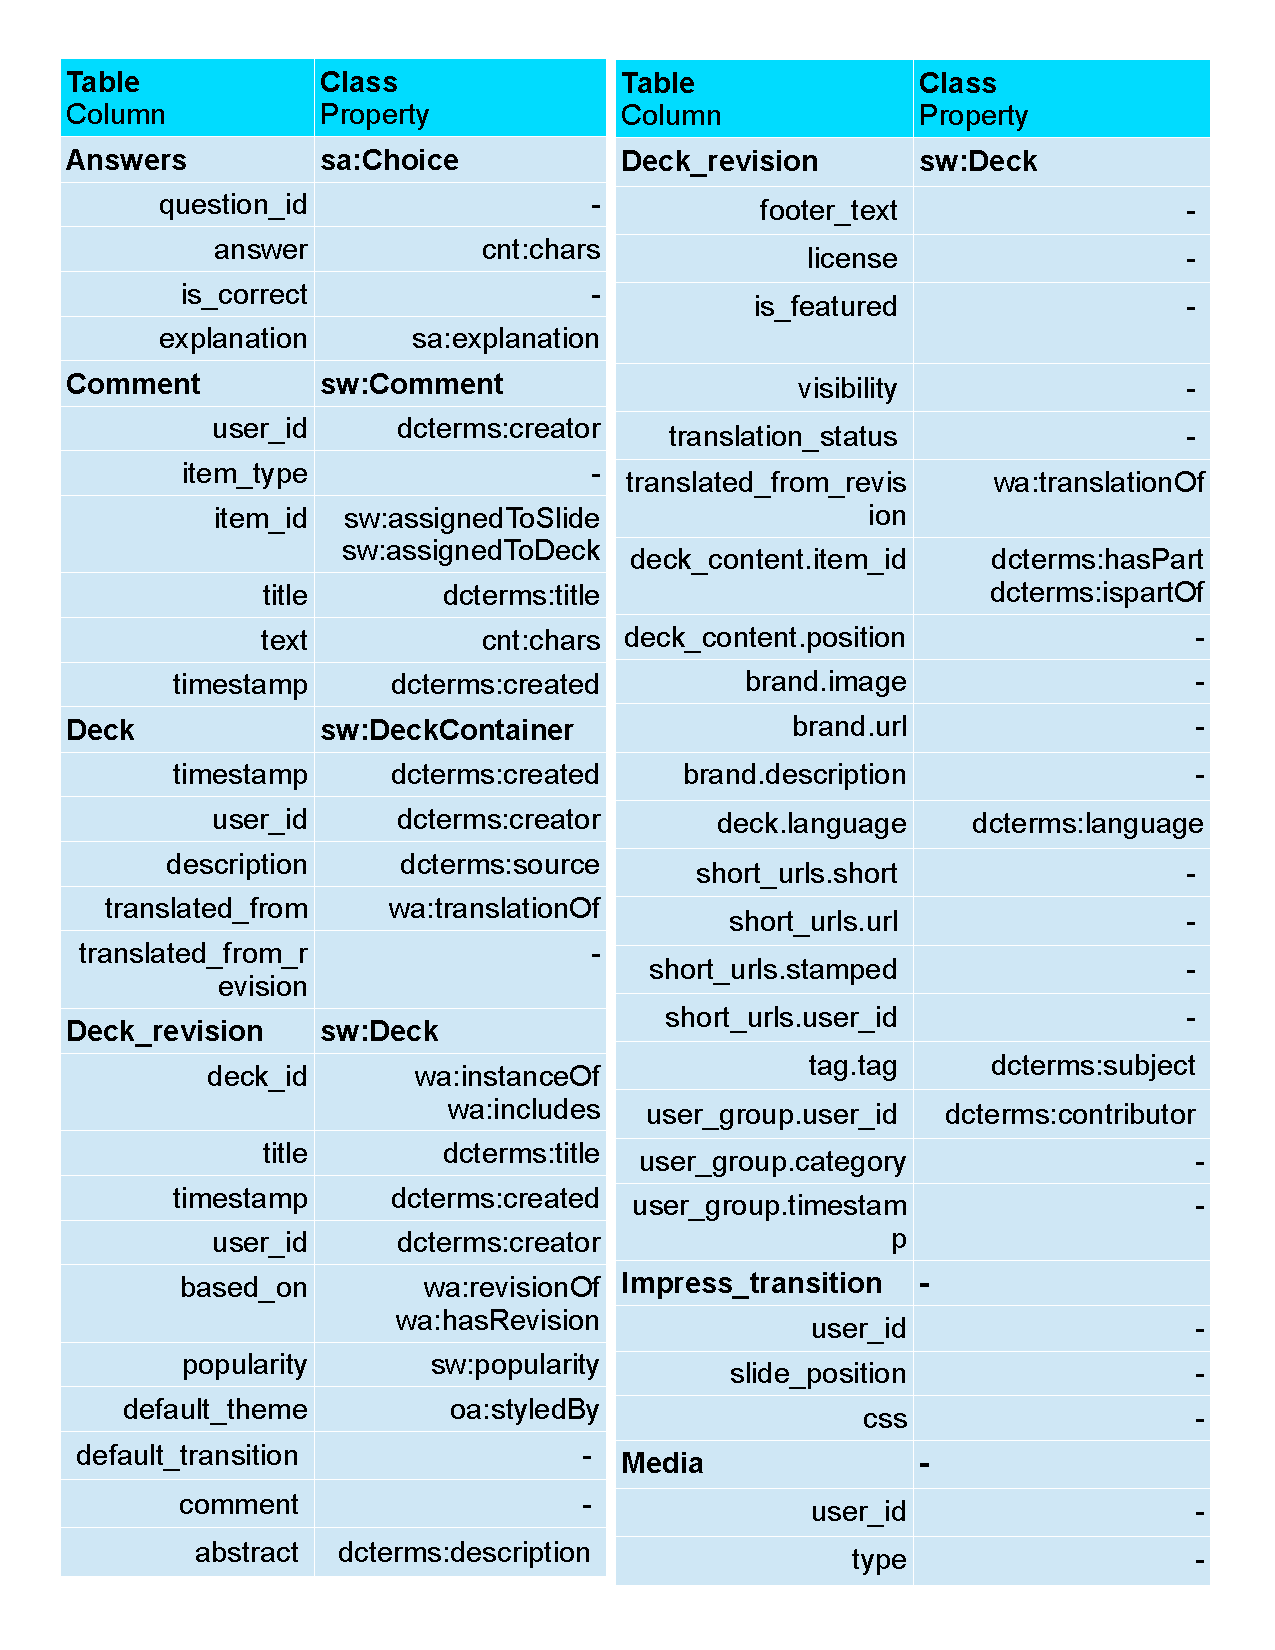
\includegraphics[width=\columnwidth]{images/mapping_pages1.pdf}
%		\caption{Matching the DB tables and columns to WikiApp ontologie classes and properties}
%	\label{fig:wa_matching_1}
%\end{figure}
%
%\begin{figure}[!b]
%	\centering
%		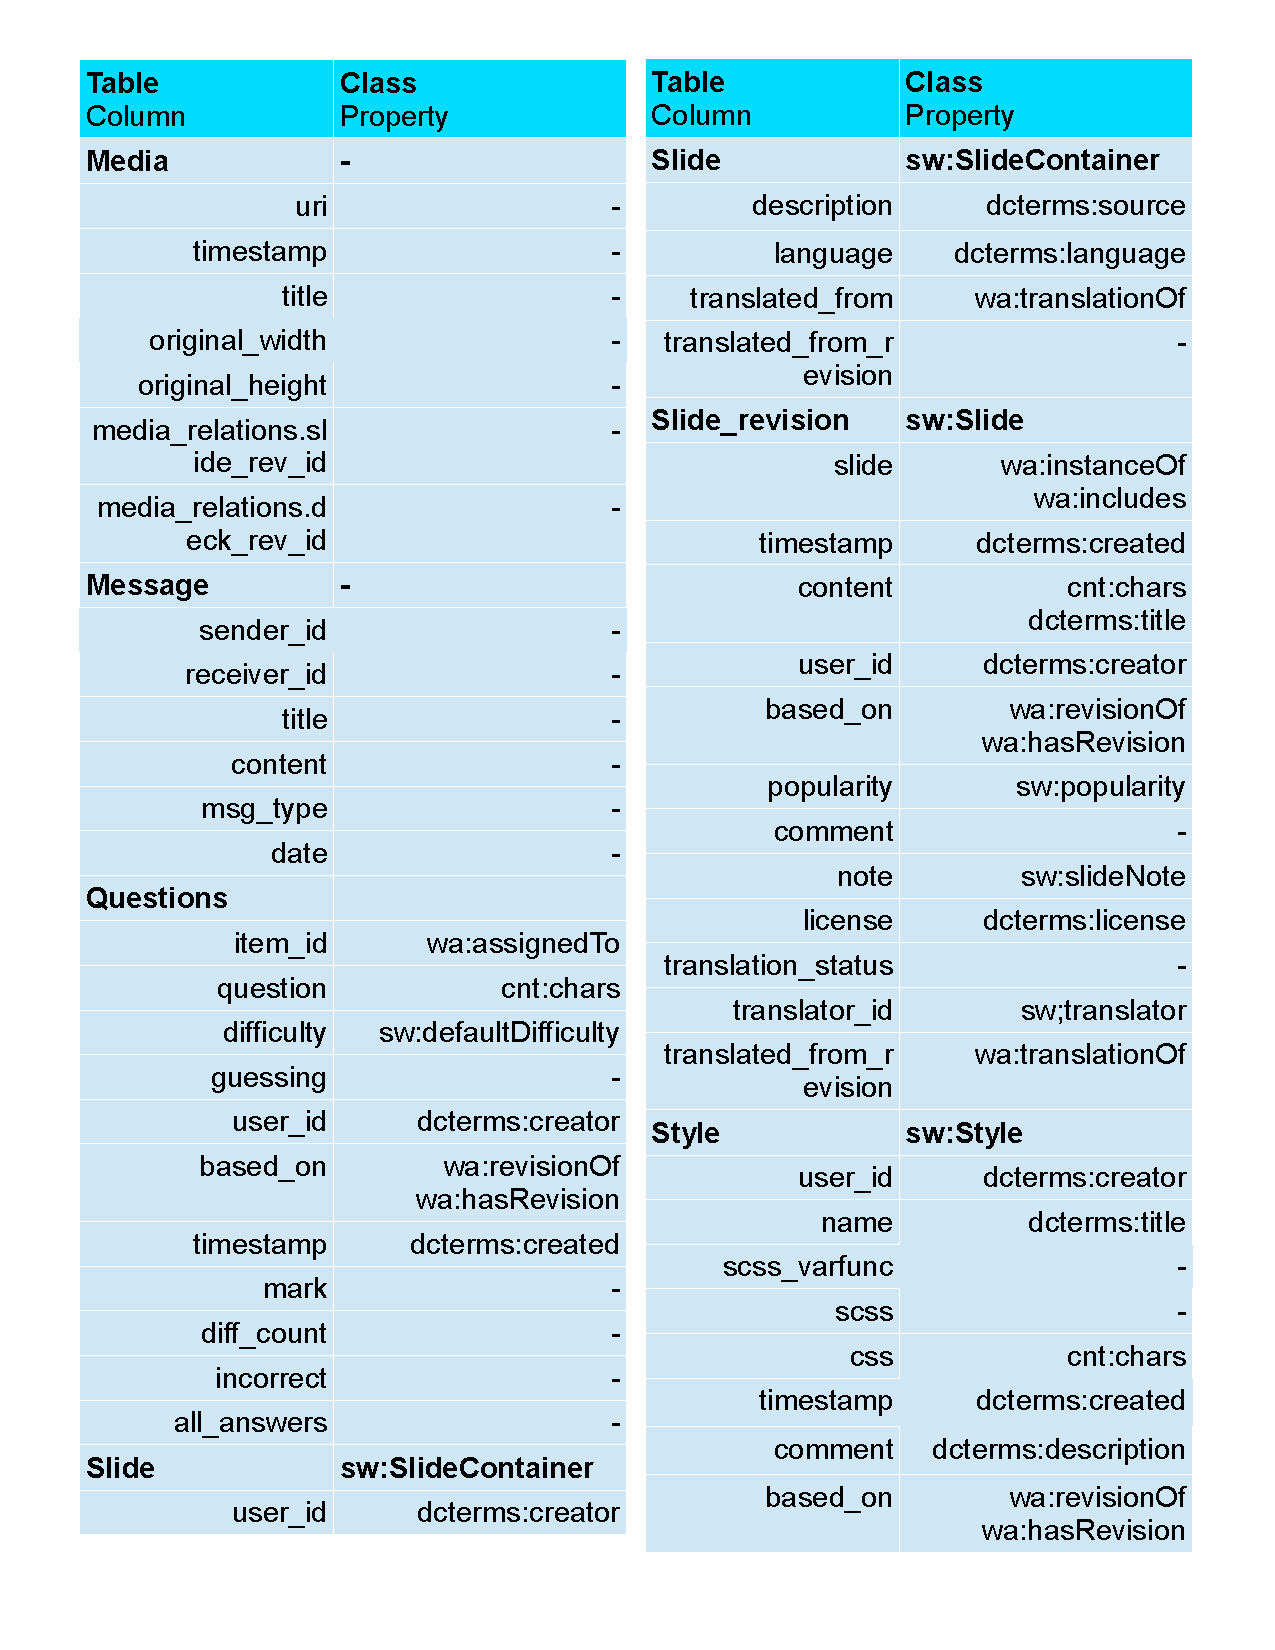
\includegraphics[width=\columnwidth]{images/mapping_pages2.pdf}
%		\caption{Matching the DB tables and columns to WikiApp ontologie classes and properties (cont.)}
%	\label{fig:wa_matching_2}
%\end{figure}
%
%\begin{figure}[!b]
%	\centering
%		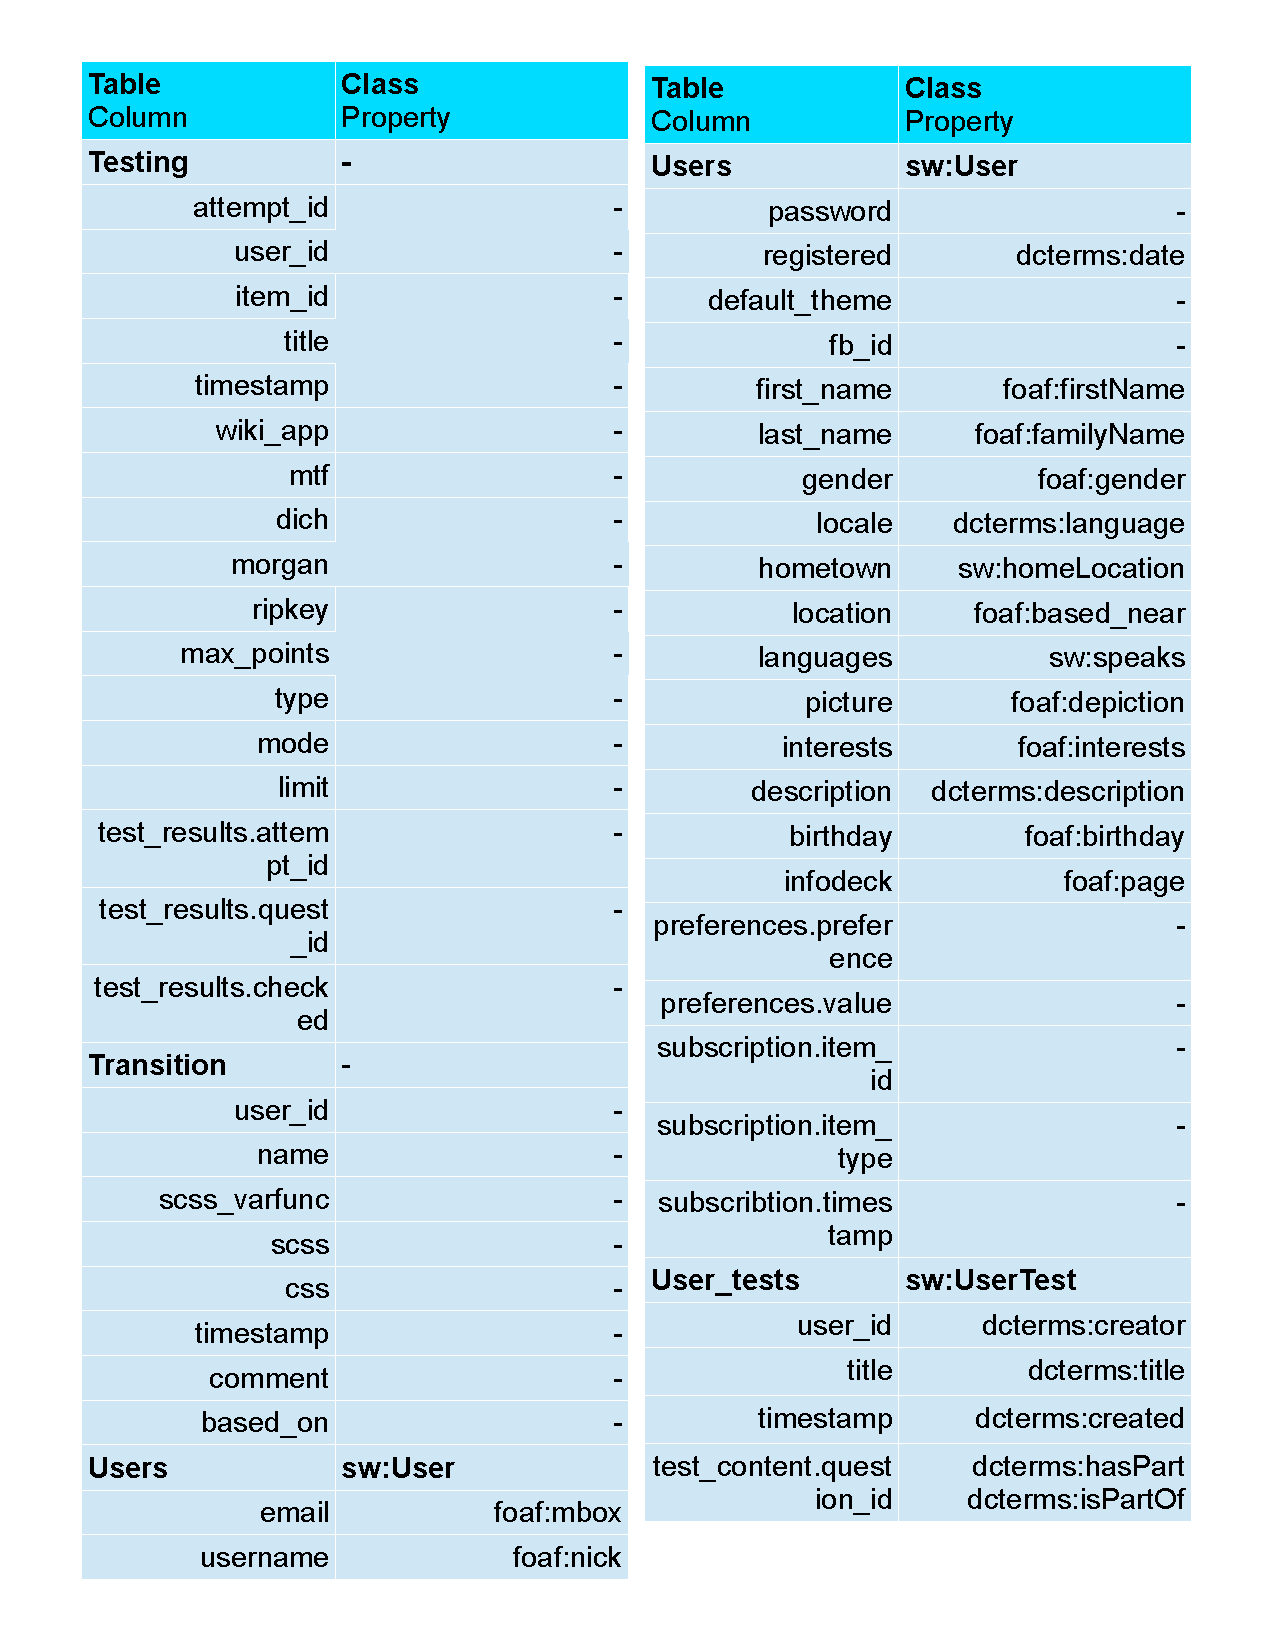
\includegraphics[width=\columnwidth]{images/mapping_pages3.pdf}
%		\caption{Matching the DB tables and columns to WikiApp ontologie classes and properties (cont.)}
%	\label{fig:wa_matching_3}
%\end{figure}


\section{SlideWiki knowledge graph}


\begin{sidewaysfigure}[b]
    \centering
    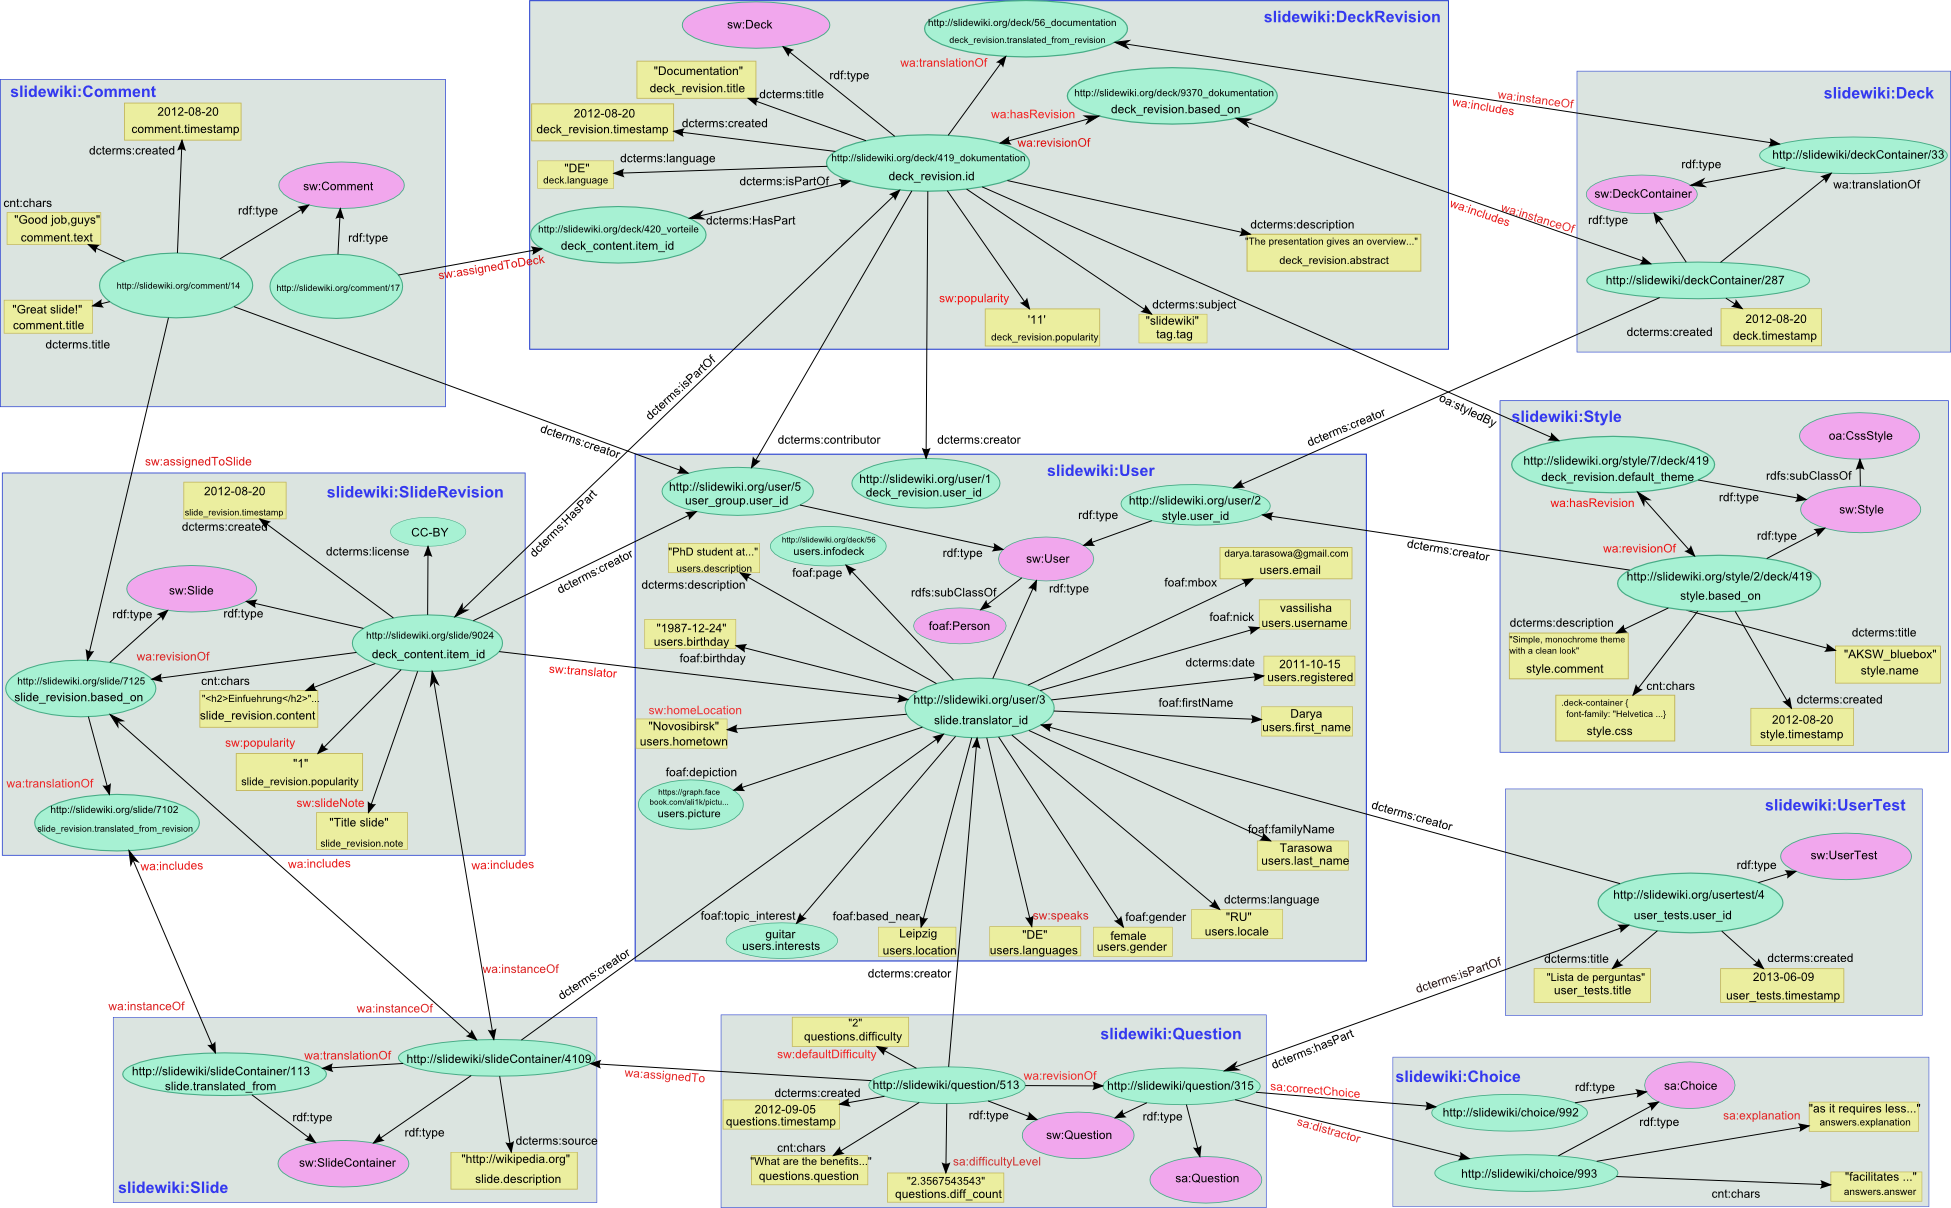
\includegraphics[width=\columnwidth]{images/knowledge_graph.png}
    \caption{SlideWiki Knowledge graph}
	\label{fig:knowledge_graph}
\end{sidewaysfigure}




